% \documentclass{standalone}
% \usepackage{tikz}
% \usepackage{multirow}
% \usetikzlibrary{shapes.geometric}
% \usetikzlibrary{decorations.pathreplacing,calligraphy}
% \usetikzlibrary{positioning}
% \usetikzlibrary{arrows.meta}
% \begin{document}

\begin{tikzpicture}[
  every node/.style={fill=white},
  base/.style={rectangle, rounded corners, draw=blue!60, fill=blue!5, very thick, minimum size=2.5cm},
  sys/.style={rectangle, rounded corners, draw=green!60, fill=green!5, very thick, minimum size=2.5cm},
  vuln/.style={rectangle, rounded corners, draw=red!60, fill=red!5, very thick, minimum size=2.5cm},
]


\node[base] (tt) {
\begin{tabular}{cc}
  \multicolumn{2}{c}{\textbf{Training \& Tuning}} \\
  \begin{tikzpicture}[
  vuln/.style={rectangle, rounded corners, draw=red!60, fill=red!5, very thick},
  ]
 \node [vuln] (v) {
    \begin{tabular}{c}
    \makebox[2cm][c]{\small Data Poisoning} \\
    \cite{11344010,11028470}
    \end{tabular}
 };
  \end{tikzpicture} &
  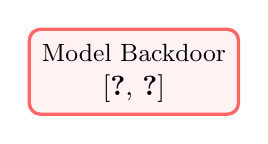
\begin{tikzpicture}[
  vuln/.style={rectangle, rounded corners, draw=red!60, fill=red!5, very thick},
  ]
 \node [vuln] (v) {
    \begin{tabular}{c}
    \makebox[2cm][c]{\small Model Backdoor} \\
    \cite{10.1016/j.infsof.2025.107707,11422005}
    \end{tabular}
 };
  \end{tikzpicture} \\
\end{tabular}
};

\node[base] (infer) [below=of tt, xshift=-3cm] {
  \begin{tabular}{cc}
  \multicolumn{2}{c}{\textbf{Inference}} \\
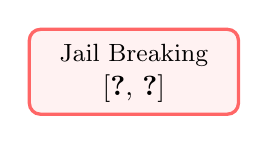
\begin{tikzpicture}[
  vuln/.style={rectangle, rounded corners, draw=red!60, fill=red!5, very thick},
  ]
 \node [vuln] (v) {
    \begin{tabular}{c}
    \makebox[2cm][c]{\small Jail Breaking} \\
    \cite{10.1007/s10515-026-00628-7,11417765}
    \end{tabular}
 };
  \end{tikzpicture} &
  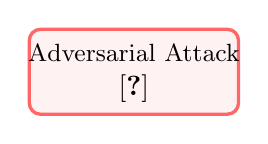
\begin{tikzpicture}[
  vuln/.style={rectangle, rounded corners, draw=red!60, fill=red!5, very thick},
  ]
 \node [vuln] (v) {
    \begin{tabular}{c}
    \makebox[2cm][c]{\small Adversarial Attack} \\
    \cite{10.1007/s10515-024-00464-7}
    \end{tabular}
 };
  \end{tikzpicture} \\
  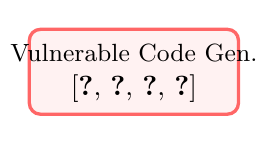
\begin{tikzpicture}[
  vuln/.style={rectangle, rounded corners, draw=red!60, fill=red!5, very thick},
  ]
 \node [vuln] (v) {
    \begin{tabular}{c}
    \makebox[2cm][c]{\small Vulnerable Code Gen.} \\
    \cite{copilotsecurity,10301242,10538871,GLAS2026104842}
    \end{tabular}
 };
  \end{tikzpicture} &
  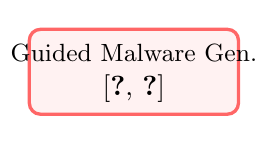
\begin{tikzpicture}[
  vuln/.style={rectangle, rounded corners, draw=red!60, fill=red!5, very thick},
  ]
 \node [vuln] (v) {
    \begin{tabular}{c}
    \makebox[2cm][c]{\small Guided Malware Gen.} \\
    \cite{ITURBE2024104077,llmbackdoordet} % improper article ID. The article leverage LLM for attacking.
    \end{tabular}
 };
  \end{tikzpicture} \\
  \multicolumn{2}{c}{
    
\begin{tikzpicture}[
  vuln/.style={rectangle, rounded corners, draw=red!60, fill=red!5, very thick},
  ]
 \node [vuln] (v) {
    \begin{tabular}{c}
    \makebox[4cm][c]{\small MLSys Breach} \\
    \cite{10.1145/3756681.3757083}
    \end{tabular}
 };
    \end{tikzpicture}
  } \\
\end{tabular}
};


\node[base] (harness) [right=of infer] {
  \begin{tabular}{cc}
  \multicolumn{2}{c}{\textbf{Agent Harness}} \\
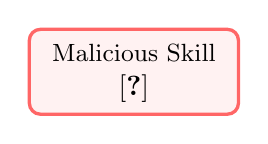
\begin{tikzpicture}[
  vuln/.style={rectangle, rounded corners, draw=red!60, fill=red!5, very thick},
  ]
 \node [vuln] (v) {
   \begin{tabular}{c}
    \makebox[2cm][c]{\small Malicious Skill} \\
    \cite{skillvulns}
   \end{tabular}
 };
  \end{tikzpicture} &
  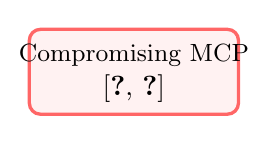
\begin{tikzpicture}[
  vuln/.style={rectangle, rounded corners, draw=red!60, fill=red!5, very thick},
  ]
 \node [vuln] (v) {
   \begin{tabular}{c}
    \makebox[2cm][c]{\small Compromising MCP} \\
    \cite{10.1145/3814959,mcpvulns}
   \end{tabular}
 };
  \end{tikzpicture} \\
  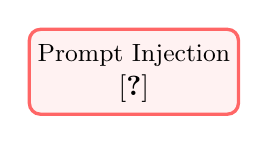
\begin{tikzpicture}[
  vuln/.style={rectangle, rounded corners, draw=red!60, fill=red!5, very thick},
  ]
 \node [vuln] (v) {
   \begin{tabular}{c}
    \makebox[2cm][c]{\small Prompt Injection} \\
    \cite{11536564}
   \end{tabular}
 };
  \end{tikzpicture} &
  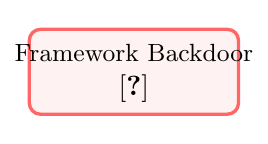
\begin{tikzpicture}[
  vuln/.style={rectangle, rounded corners, draw=red!60, fill=red!5, very thick},
  ]
 \node [vuln] (v) {
   \begin{tabular}{c}
    \makebox[2cm][c]{\small Framework Backdoor} \\
    \cite{11536564}
   \end{tabular}
 };
  \end{tikzpicture}  \\

  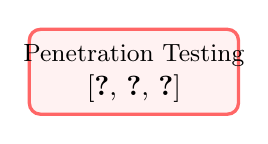
\begin{tikzpicture}[
  vuln/.style={rectangle, rounded corners, draw=red!60, fill=red!5, very thick},
  ]
 \node [vuln] (v) {
  \begin{tabular}{c}
    \makebox[2cm][c]{\small Penetration Testing} \\
    \cite{10970188,11418046,10.1145/3766895}
  \end{tabular}
 };
  \end{tikzpicture} &
  
\begin{tikzpicture}[
  vuln/.style={rectangle, rounded corners, draw=red!60, fill=red!5, very thick},
  ]
 \node [vuln] (v) {
    \begin{tabular}{c}
    \makebox[2cm][c]{\small Social Engineering} \\
    \cite{10187385}
    \end{tabular}
 };
  \end{tikzpicture} 
\end{tabular}
};

\end{tikzpicture}
% \end{document}
